\documentclass{article}

% if you need to pass options to natbib, use, e.g.:
%     \PassOptionsToPackage{numbers, compress}{natbib}
% before loading neurips_2026

% The authors should use one of these tracks.
% Before accepting by the NeurIPS conference, select one of the options below.
% 0. "default" for submission
% \usepackage{neurips_2026}
% the "default" option is equal to the "main" option, which is used for the Main Track with double-blind reviewing.
% 1. "main" option is used for the Main Track
 % For anonymized double-blind submission: use [main] only. The [final] option
 % reveals author names and is reserved for the camera-ready version.
  \usepackage[main]{neurips_2026}
 % \usepackage[main, final]{neurips_2026}
% 2. "position" option is used for the Position Paper Track
%  \usepackage[position]{neurips_2026}
% 3. "eandd" option is used for the Evaluations & Datasets Track
 % \usepackage[eandd]{neurips_2026}
 % if you need to opt-in for a single-blind submission in the E&D track:
 %\usepackage[eandd, nonanonymous]{neurips_2026}
% 4. "creativeai" option is used for the Creative AI Track
%  \usepackage[creativeai]{neurips_2026}
% 5. "sglblindworkshop" option is used for the Workshop with single-blind reviewing
 % \usepackage[sglblindworkshop]{neurips_2026}
% 6. "dblblindworkshop" option is used for the Workshop with double-blind reviewing
%  \usepackage[dblblindworkshop]{neurips_2026}

% After being accepted, the authors should add "final" behind the track to compile a camera-ready version.
% 1. Main Track
 % \usepackage[main, final]{neurips_2026}
% 2. Position Paper Track
%  \usepackage[position, final]{neurips_2026}
% 3. Evaluations & Datasets Track
 % \usepackage[eandd, final]{neurips_2026}
% 4. Creative AI Track
%  \usepackage[creativeai, final]{neurips_2026}
% 5. Workshop with single-blind reviewing
%  \usepackage[sglblindworkshop, final]{neurips_2026}
% 6. Workshop with double-blind reviewing
%  \usepackage[dblblindworkshop, final]{neurips_2026}
% Note. For the workshop paper template, both \title{} and \workshoptitle{} are required, with the former indicating the paper title shown in the title and the latter indicating the workshop title displayed in the footnote.
% For workshops (5., 6.), the authors should add the name of the workshop, "\workshoptitle" command is used to set the workshop title.
% \workshoptitle{WORKSHOP TITLE}

% "preprint" option is used for arXiv or other preprint submissions
 % \usepackage[preprint]{neurips_2026}

% to avoid loading the natbib package, add option nonatbib:
%    \usepackage[nonatbib]{neurips_2026}

\usepackage[utf8]{inputenc} % allow utf-8 input
\usepackage[T1]{fontenc}    % use 8-bit T1 fonts
\usepackage{hyperref}       % hyperlinks
\usepackage{url}            % simple URL typesetting
\usepackage{booktabs}       % professional-quality tables
\usepackage{amsmath}        % environments like align, equation*
\usepackage{amsfonts}       % blackboard math symbols
\usepackage{amssymb}        % additional math symbols
\usepackage{nicefrac}       % compact symbols for 1/2, etc.
\usepackage{microtype}      % microtypography
\usepackage{xcolor}         % colors
\usepackage{graphicx}
\usepackage{algorithm}      % algorithm floats
\usepackage{algpseudocode}  % algorithmic environment

% Note. For the workshop paper template, both \title{} and \workshoptitle{} are required, with the former indicating the paper title shown in the title and the latter indicating the workshop title displayed in the footnote. 
\title{Composable Energy Policies: Zero-Shot Per-Agent Constraint Adaptation in Multi-Agent Control}


% The \author macro works with any number of authors. There are two commands
% used to separate the names and addresses of multiple authors: \And and \AND.
%
% Using \And between authors leaves it to LaTeX to determine where to break the
% lines. Using \AND forces a line break at that point. So, if LaTeX puts 3 of 4
% authors names on the first line, and the last on the second line, try using
% \AND instead of \And before the third author name.


\author{%
  Marcus Binder Nilsen \thanks{Use footnote for providing further information
    about author (webpage, alternative address)---\emph{not} for acknowledging
    funding agencies.} \\
  Department of Wind and Energy Systems\\
  Technical University of Denmark \\
  Roskilde, Frederiksborgvej 399 \\
  \texttt{manils@dtu.dk} \\
  % examples of more authors
  \And
  Julian Quick  \\
  Department of Wind and Energy Systems\\
  Technical University of Denmark \\
  Roskilde, Frederiksborgvej 399 \\
  \texttt{juqu@dtu.dk} \\
  % \AND
  % Coauthor \\
  % Affiliation \\
  % Address \\
  % \texttt{email} \\
  % \And
  % Coauthor \\
  % Affiliation \\
  % Address \\
  % \texttt{email} \\
  % \And
  % Coauthor \\
  % Affiliation \\
  % Address \\
  % \texttt{email} \\
}


\begin{document}


\maketitle


\begin{abstract}
Deploying reinforcement-learning policies in multi-agent physical systems requires adapting to operational constraints that change over a system's lifetime: per-agent fatigue budgets across multiple damage channels, travel limits, maintenance exclusions. Existing constrained-RL methods force operators to retrain the entire team for every new constraint configuration, and single-agent composable-energy methods cannot express the cross-agent reallocation that arises when constraints affect only a subset of teammates. We introduce \emph{Composable Energy Policies for Multi-Agent Control}, an energy-based transformer actor trained by soft actor--critic in which each agent is a token and the policy exposes an explicit per-token energy $E(s, a_i)$. At deployment, arbitrary differentiable per-agent $\times$ per-channel constraint energies compose additively, and gradient-based joint optimization produces \emph{joint re-optimization at inference time}: constraining one token causes unconstrained teammates to reallocate their actions to a new joint optimum that respects every channel budget. We quantify the effect with a \emph{Counterfactual Displacement Ratio} (CDR) that is exactly zero for action clipping, bounded-small for a Gaussian actor with penalty-gradient refinement, and $\Omega(1)$ for our method. On wind-farm yaw control with real neural damage-equivalent-load surrogates, a single policy traces Pareto frontiers across multiple fatigue channels at zero retraining cost, approximately matching per-weighting Lagrangian-retrained baselines. We map a $(\text{coupling strength} \times \text{constraint strength} \times \text{channel})$ phase diagram characterizing when composition recovers the retrained optimum and when it degenerates to clipping. Two architectural ablations---replacing per-token energies with a farm-level scalar head, and stripping cross-agent attention from the backbone---each eliminate the reallocation effect, isolating it as a structural property of \emph{per-token multi-agent} energy composition rather than of explicit energy composition alone.
\end{abstract}


\section{Introduction}
\label{sec:introduction}
Here is 1-1.5 pages: Motivate the problem, state your contribution clearly (often as a numbered list of 2–4 contributions), and briefly preview the results. Reviewers often form their initial impression here, so it needs to land.

\begin{figure}
    \centering
    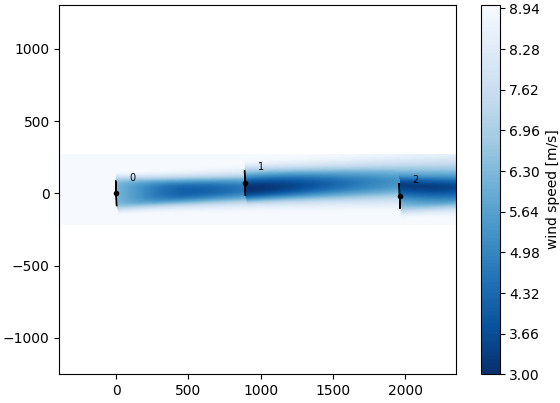
\includegraphics[width=0.75\linewidth]{figs/image.png}
    \caption{Flow field of the farm}
    \label{fig:farm}
\end{figure}


\begin{figure}
    \centering
    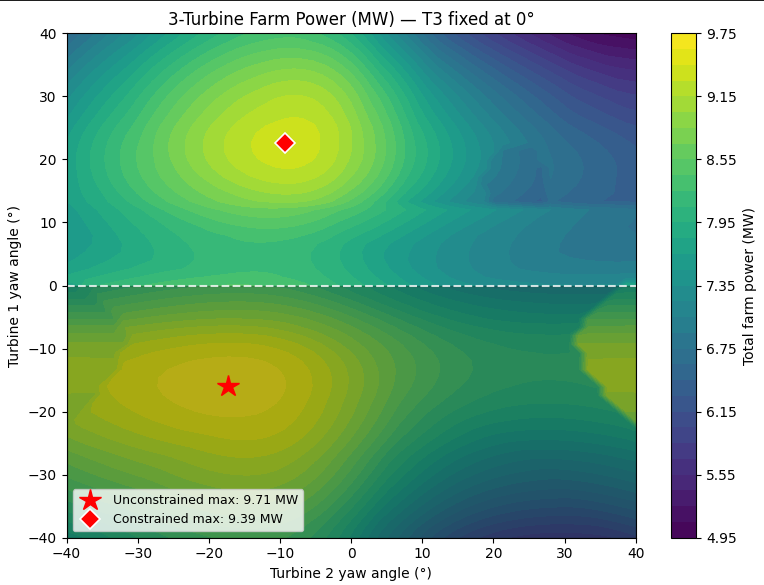
\includegraphics[width=0.75\linewidth]{figs/landscape.png}
    \caption{Contour plot of the power output of the farm}
    \label{fig:powersurface}
\end{figure}



\section{Related work}
\label{sec:related}
0.5-1 page: Can appear here or later (before the conclusion). Position your work relative to existing literature. The goal is to show you know the landscape and to clearly differentiate your contribution. For your project, this would cover EBMs in RL, composable energy functions, wind farm control with RL, and safety-constrained policy optimization.


\section{Background}
\label{sec:background}

\paragraph{Cooperative multi-agent control.}
We consider a cooperative Markov game with $N$ agents whose joint action is $a = (a_1, \ldots, a_N) \in \mathcal{A}_1 \times \cdots \times \mathcal{A}_N$, a shared state $s$, and a shared reward $r(s, a)$. The number of agents $N$ can vary between episodes (e.g., across farm layouts), which motivates a set-structured policy that generalizes across $N$. In what follows we use \emph{agent} and \emph{turbine} interchangeably when discussing the wind-farm instantiation.

\paragraph{Maximum-entropy RL and its energy-based reading.}
Soft actor--critic (SAC)~\citep{sac_haarnoja2018} optimizes the entropy-regularized objective $J(\pi) = \mathbb{E}_\pi\!\left[\sum_t r(s_t, a_t) + \alpha\, \mathcal{H}(\pi(\cdot \mid s_t))\right]$. The optimal policy is the Boltzmann distribution over the soft Q-function,
\begin{equation}
\pi^*(a \mid s) \;\propto\; \exp\!\left(Q^*(s, a) / \alpha\right),
\label{eq:boltzmann}
\end{equation}
which is an energy-based model with \emph{energy} $E(s, a) \coloneqq -Q^*(s, a)/\alpha$~\citep{sql_haarnoja2017}. The actor in standard SAC is a reparameterized squashed Gaussian: tractable but unimodal, and the explicit energy is discarded. Making the energy explicit again recovers multimodality and---crucially for this work---\emph{compositionality}, at the cost of replacing closed-form sampling with iterative optimization.

\paragraph{Constrained RL and Lagrangian relaxation.}
Given a task objective $E_\text{task}$ and inequality constraints $E_c(a) \leq b_c$ for $c = 1, \ldots, C$, the constrained optimization problem
\begin{equation}
\min_a\; E_\text{task}(a) \quad \text{s.t.} \quad E_c(a) \leq b_c,\; c=1, \ldots, C
\label{eq:constrained}
\end{equation}
admits the Lagrangian relaxation $L(a, \lambda) = E_\text{task}(a) + \sum_c \lambda_c \bigl(E_c(a) - b_c\bigr)$ with non-negative multipliers $\lambda_c \geq 0$. Under strong duality, sweeping $\lambda \in \mathbb{R}^C_{\geq 0}$ traces the Pareto frontier of \eqref{eq:constrained}. For differentiable $E_c$, unconstrained minimization of $L$ at a fixed $\lambda$ is exactly what an energy-based policy does when $E_\text{task}$ and the $E_c$ are combined additively and optimized jointly. This identification has been used for single-agent safe diffusion~\citep{algd2026}; the contribution of this paper is not the identification itself but (i) its \emph{multi-agent} instantiation and (ii) the empirical characterization of when post-hoc Lagrangian composition at a pretrained energy recovers the retrained optimum.


\section{Methodology}
\label{sec:methodology}

We build Composable Energy Policies for Multi-Agent Control (\textbf{CEP-MA}) on three ingredients: a transformer backbone that tokenizes agents~(Sec.~\ref{sec:method:backbone}), an energy-based actor head trained by a soft actor--critic objective~(Sec.~\ref{sec:method:energy},~\ref{sec:method:training}), and a post-hoc rule for composing per-agent per-channel constraint energies at deployment~(Sec.~\ref{sec:method:composition}).

\subsection{Transformer backbone: agents as tokens}
\label{sec:method:backbone}

Each agent $i$ is associated with an observation $o_i \in \mathbb{R}^{d_o}$ (local wind field, own action history, neighbor-relative positions) and a spatial descriptor $p_i$ (position in the farm, rotor diameter, wake-influence profile). We first map $o_i$ to an embedding token $z_i^0 = \phi_\text{obs}(o_i) + \phi_\text{pos}(p_i)$, where $\phi_\text{pos}$ is one of several spatial positional encodings discussed in the appendix. Positions are expressed in a \emph{wind-relative frame} so that the encoded spatial structure is invariant to wind-direction rotation.

A stack of $L$ transformer encoder layers with multi-head self-attention over the $N$ tokens produces contextual embeddings $z_i = \operatorname{Transformer}(z_1^0, \ldots, z_N^0)_i$. Because the backbone processes a variable-length sequence, a single trained model applies to farms of arbitrary size without architectural changes---enabling zero-shot generalization to unseen $N$.

\subsection{Energy-based actor head}
\label{sec:method:energy}

The actor head is a shared-weight MLP $f_E$ that scores a candidate action $a_i \in \mathcal{A}_i$ against its contextual embedding:
\begin{equation}
E_i(s, a_i) \;=\; f_E\!\left([\,z_i\,;\,a_i\,]\right) \in \mathbb{R},
\qquad
E(s, a) \;=\; \sum_{i=1}^{N} E_i(s, a_i).
\label{eq:energy}
\end{equation}
Lower energy corresponds to more compatible actions. Following~\eqref{eq:boltzmann}, the implicit policy is $\pi_\theta(a \mid s) \propto \exp\!\left(-E(s, a)\right)$, with the temperature absorbed into the energy scale.

Note that while the per-token energies $E_i$ are computed through a shared MLP, the embeddings $z_i$ are cross-coupled through the transformer's self-attention: $z_i$ depends on \emph{all} $o_j$ and $p_j$. Consequently, $E(s, a)$ is not separable over $a$ at the level of its derivatives---adding a term that touches only $a_i$ will, in general, shift the joint minimizer in every coordinate. This is the structural property that produces cooperative reorganization in Sec.~\ref{sec:method:composition}, and it is the property a single-agent composable-energy method~\citep{cep_urain2023, ebt_policy2025} cannot express because it lacks the joint token embedding.

\subsection{Action generation via gradient descent with self-verification}
\label{sec:method:inference}

Given a state $s$, we generate an action by minimizing $E(s, a)$ jointly over all tokens. Following the Energy-Based Transformer procedure~\citep{ebt_base2025, ebt_policy2025}, we combine \emph{self-verification} (sampling $M$ candidates) with gradient-based refinement (running $K$ optimization steps per candidate):
\begin{algorithm}[t]
\caption{Action generation with self-verification (single step)}
\label{alg:infer}
\begin{algorithmic}[1]
\Require state $s$, candidates $M$, refinement steps $K$, step size $\eta$, composed energy $\widetilde E(s, \cdot)$
\For{$m = 1, \ldots, M$}
    \State $a_m^{(0)} \sim \mathcal{U}(\mathcal{A})$ \Comment{or Gaussian prior}
    \For{$k = 0, \ldots, K-1$}
        \State $a_m^{(k+1)} \gets \operatorname{Proj}_{\mathcal{A}}\!\left(a_m^{(k)} - \eta\, \nabla_a \widetilde E(s, a_m^{(k)})\right)$
    \EndFor
\EndFor
\State \Return $a^\star = \operatorname*{arg\,min}_{m}\, \widetilde E\!\left(s, a_m^{(K)}\right)$
\end{algorithmic}
\end{algorithm}
Crucially, both $M$ and $K$ are knobs at inference time only: more candidates or more steps trade compute for action quality, and neither requires retraining. In training, $\widetilde E = E$ is the actor energy; at deployment it is extended with constraint energies (Sec.~\ref{sec:method:composition}).

\subsection{Training: SAC with an explicit energy head}
\label{sec:method:training}

We train the backbone and energy head jointly with a variant of SAC adapted to the explicit energy formulation.  A twin-Q critic is trained as in standard SAC via the Bellman target on transitions from a replay buffer; we refer to the appendix for details. The actor objective is the maximum-entropy policy improvement:
\begin{equation}
\mathcal{L}_\text{actor}(\theta) \;=\; \mathbb{E}_{s \sim \mathcal{D}}\!\left[\mathbb{E}_{a \sim \pi_\theta(\cdot|s)}\!\left[\alpha \log \pi_\theta(a \mid s) - Q(s, a)\right]\right].
\label{eq:sac-actor}
\end{equation}
For a reparameterized squashed Gaussian, $\log \pi_\theta$ is tractable. For our energy-based policy $\pi_\theta(a \mid s) \propto \exp(-E(s, a))$, however, $\log \pi_\theta(a \mid s) = -E(s, a) - \log Z(s)$ requires the partition function $Z(s)$. We estimate it by self-normalizing importance sampling over the very same self-verification candidates used at inference:
\begin{equation}
\log Z(s) \;\approx\; \operatorname{LogSumExp}_{m = 1, \ldots, M}\!\left(-E\!\left(s, a_m^{(K)}\right)\right) + \log\frac{|\mathcal{A}|}{M},
\label{eq:logz}
\end{equation}
where the $a_m^{(K)}$ are produced by Alg.~\ref{alg:infer} with $\widetilde E = E$. Substituting \eqref{eq:logz} into \eqref{eq:sac-actor} yields a well-defined actor loss that back-propagates through both the energy scores and the critic. This simultaneously recovers a maximum-entropy training signal for the energy and stays consistent with the inference procedure.

\subsection{Post-hoc composition of per-agent per-channel constraint energies}
\label{sec:method:composition}

At deployment, an operator specifies a set of differentiable \emph{constraint energies}
$\bigl\{\,E_{i,c}: \mathcal{A}_i \times \mathcal{S} \to \mathbb{R}_{\geq 0}\,\bigr\}_{i \in \mathcal{I}, c \in \mathcal{C}}$
indexed by agent subsets $\mathcal{I} \subseteq \{1, \ldots, N\}$ and damage or safety channels $\mathcal{C}$. Each $E_{i,c}$ is non-negative, zero inside its safe region, and increases smoothly outside. Multipliers $\lambda_{i,c} \geq 0$ encode the operator's relative priorities. The \emph{composed energy} at deployment is
\begin{equation}
\widetilde E(s, a) \;=\; E(s, a) \;+\; \sum_{i \in \mathcal{I}} \sum_{c \in \mathcal{C}} \lambda_{i,c} \cdot E_{i,c}(a_i, s).
\label{eq:composition}
\end{equation}
Action generation at deployment is Alg.~\ref{alg:infer} applied to $\widetilde E$. No parameters of the trained actor, critic, or backbone change.

Equation~\eqref{eq:composition} is the Lagrangian relaxation of
\begin{equation}
\min_a\; E(s, a) \quad \text{s.t.}\quad E_{i,c}(a_i, s) \leq 0\; \text{for all } (i, c) \in \mathcal{I} \times \mathcal{C},
\label{eq:deployed-constrained}
\end{equation}
where the $\lambda_{i,c}$ play the role of dual variables. Under convexity assumptions and strong duality, sweeping $\lambda$ traces the Pareto frontier of~\eqref{eq:deployed-constrained}; in realistic non-convex settings, the quality of this correspondence is an empirical question that we address in Sec.~\ref{sec:experiments} with a $(\text{coupling strength} \times \text{constraint strength} \times \text{channel})$ phase diagram. This theoretical identification is not itself a contribution---it has been made for single-agent safe diffusion~\citep{algd2026}---but the multi-agent instantiation and its empirical envelope are.

\paragraph{Why composition yields \emph{cooperative} reorganization.}
Because the trained energy $E$ is not separable in $a$ (Sec.~\ref{sec:method:energy}), the joint minimizer $a^\star = \operatorname*{arg\,min}_a \widetilde E(s, a)$ can differ from the unconstrained $a^\circ = \operatorname*{arg\,min}_a E(s, a)$ in \emph{every} coordinate, not just the coordinates touched by $E_{i,c}$. Concretely, adding a penalty on $a_i$ shifts the level sets of $\widetilde E$ along the $a_i$ axis; minimizing the shifted energy jointly over all agents then propagates the change to $a_j$ for $j \neq i$ whenever $\partial^2 E / \partial a_i \partial a_j \neq 0$ somewhere on the optimization path. This cross-derivative is created by the transformer's cross-token attention: $z_j$ depends on $o_i$, and therefore $E_j(s, a_j) = f_E([z_j; a_j])$ inherits a dependence on $o_i$ that, at test time, makes $a_j^\star$ sensitive to constraints placed on agent $i$. An ablation that replaces the attention-based backbone with independent per-agent encoders (Sec.~\ref{sec:experiments}) breaks the cross-derivative and eliminates the reorganization, isolating it as a structural property of \emph{multi-agent} energy composition rather than of explicit energy composition per se.

\paragraph{Heterogeneous per-agent per-channel constraints.}
A key practical consequence is that~\eqref{eq:composition} admits arbitrary heterogeneous constraint profiles at zero extra training cost. An operator can, for example, place a strict tower-base fatigue budget on an aging turbine and a looser blade-root budget on a recently inspected one, mix in a global yaw-travel budget, and exclude a turbine from maintenance-time yawing---all by populating $\lambda_{i,c}$ and $E_{i,c}$. Alg.~\ref{alg:infer} responds with a joint action that trades off every listed objective simultaneously, and setting any $\lambda_{i,c} = 0$ exactly recovers the unconstrained behavior along that dimension.

\subsection{Measuring joint re-optimization: the Counterfactual Displacement Ratio}
\label{sec:method:cdr}

The phrase ``cooperative reorganization'' is operationally ambiguous. A trivial joint optimizer over a separable energy reorganizes nothing---each coordinate minimizes independently---and yet, by the letter of the description, the free coordinates ``change'' whenever the constrained coordinate changes if they share any spurious correlation with it. We need a metric that distinguishes action clipping (which changes only the constrained coordinates) from a bounded penalty-based refinement (which moves the free coordinates a small amount away from the trained mean) from genuine cooperative re-optimization (which moves them by an amount comparable to the forced move on the constrained coordinate).

\paragraph{Definition.}
Given an unconstrained joint action $a^\circ = \operatorname*{arg\,min}_a E(s, a)$ and the composed-constrained action $a^\star = \operatorname*{arg\,min}_a \widetilde E(s, a)$ produced by Alg.~\ref{alg:infer} under~\eqref{eq:composition}, let $\mathcal{I}$ be the indices of constrained agents and $\bar{\mathcal{I}}$ its complement. We define the \emph{Counterfactual Displacement Ratio}
\begin{equation}
\mathrm{CDR}\!\left(a^\circ, a^\star\right) \;=\; \frac{\left\lVert a^\star_{\bar{\mathcal{I}}} - a^\circ_{\bar{\mathcal{I}}} \right\rVert_2}{\left\lVert a^\star_{\mathcal{I}} - a^\circ_{\mathcal{I}} \right\rVert_2 + \varepsilon}.
\label{eq:cdr}
\end{equation}
The numerator measures how much unconstrained teammates move in response to the constraint; the denominator normalizes by the move forced on the constrained agent itself, so the metric is scale-invariant in $\lambda$ and comparable across constraint types. A small additive $\varepsilon > 0$ is used when a constraint leaves the constrained coordinates near the unconstrained value.

\paragraph{Predicted regimes.}
Eq.~\eqref{eq:cdr} partitions the space of constrained policies into three regimes that differ in both mechanism and expected value:
\begin{itemize}
  \item \textbf{Action clipping.} Projecting the constrained coordinates onto the feasible set leaves $a^\star_{\bar{\mathcal{I}}} = a^\circ_{\bar{\mathcal{I}}}$, so $\mathrm{CDR} = 0$ \emph{by construction}. The free coordinates are untouched, and whatever cooperative benefit exists is missed.
  \item \textbf{Gaussian actor with penalty-gradient refinement.} A standard Gaussian SAC actor with inference-time gradient steps on $-\log \pi_\theta(a \mid s) + \lambda C(a)$ starting from the Gaussian mean yields $\mathrm{CDR}$ bounded by the actor's quadratic curvature away from its trained mean. In practice the free coordinates stay within a few degrees of their unconstrained values, so $\mathrm{CDR}$ is small but nonzero.
  \item \textbf{Composable energy policies (ours).} When $E(s, a)$ is non-separable in $a$---i.e., when the cross-derivative $\partial^2 E / \partial a_i \partial a_j$ is nontrivial, as it is when cross-token attention couples $z_i$ to all $o_j$---the joint minimizer of $\widetilde E$ differs from $a^\circ$ in every coordinate. We expect and confirm $\mathrm{CDR} = \Omega(1)$.
\end{itemize}
CDR thus serves both as a headline metric reported alongside power and per-channel DELs in Sec.~\ref{sec:experiments}, and as a diagnostic for two architectural ablations (farm-level energy head, cross-agent attention removed) that each should collapse it toward zero and thereby isolate the mechanism.

\section{Experiments}
\label{sec:experiments}
2-3 pages: Empirical validation. Typical subsections include the experimental setup (simulator details, baselines, metrics), main results (tables/figures comparing against baselines), and ablations (what happens if you remove composability, vary $\lambda$, change the number of refinement steps, etc.). For NeurIPS, reviewers expect rigorous ablations and error bars.

\section{Analysis/Discussion}
\label{sec:disc}
0.5-1 page: Optional but valuable. Deeper dives into why things work, failure modes, computational cost analysis, limitations. Being upfront about limitations (like single-domain evaluation) actually builds credibility.

\section{Conclusion}
\label{sec:conc}
0.5 pages: Summarize contributions, acknowledge limitations, gesture at future work. Keep it brief.




\begin{ack}
Use unnumbered first level headings for the acknowledgments. All acknowledgments
go at the end of the paper before the list of references. Moreover, you are required to declare
funding (financial activities supporting the submitted work) and competing interests (related financial activities outside the submitted work).
More information about this disclosure can be found at: \url{https://neurips.cc/Conferences/2026/PaperInformation/FundingDisclosure}.


Do {\bf not} include this section in the anonymized submission, only in the final paper. You can use the \texttt{ack} environment provided in the style file to automatically hide this section in the anonymized submission.
\end{ack}

\section*{References}



%%%%%%%%%%%%%%%%%%%%%%%%%%%%%%%%%%%%%%%%%%%%%%%%%%%%%%%%%%%%

\appendix

\section{Technical appendices and supplementary material}
Technical appendices with additional results, figures, graphs, and proofs may be submitted with the paper submission before the full submission deadline (see above). You can upload a ZIP file for videos or code, but do not upload a separate PDF file for the appendix. There is no page limit for the technical appendices. 

Note: Think of the appendix as ``optional reading'' for reviewers. The paper must be able to stand alone without the appendix; for example, adding critical experiments that support the main claims to an appendix is inappropriate. 

%%%%%%%%%%%%%%%%%%%%%%%%%%%%%%%%%%%%%%%%%%%%%%%%%%%%%%%%%%%%

\newpage
\input{checklist.tex}


\end{document}